\documentclass{./settings/pracamgr}
\usepackage{./settings/mystyle}

\author{Mateusz Łącki}
\nralbumu{39885}
\title{Własności algorytmu Parallel Tempering.}	
\tytulang{Properties of the Parallel Tempering algorithm.}
\kierunek{Matematyka}

\opiekun{
	{dra Błażeja Miasojedowa}	\\
	Zakład Statystyki Matematycznej.\\
}
\date{Czerwiec 2013}

\dziedzina{	11.2 Statystyka }
\klasyfikacja{ ACM I.6.7.}


\keywords{Parallel Tempering, Metropolis-Hastings, Stochastic Simulations, R}


\begin{document}

	\maketitle
%\renewcommand\bibname{Spis literatury}	
	
	\begin{abstract}
Parallel Tempering (PT) is an extension to standard Metropolis-Hastings (MH) algorithm for simulating samples from a given distribution. The standard MH algorithm with high probability remains a local algorithm, in the sense that samples are drawn from some local probability mass cluster. This is highly problematic in case of multimodial distributions that frequently appear in applications, i.e. in bayesian hierarchical models. The PT algorithm is one of most celebrated possible solutions to that problem. 

Here we present a newly developed template for running simulations written in the R statistical programming language. Being highly modular it provides a general tool for performing simulations with many user provided state-spaces.
\end{abstract}

	\setcounter{page}{1}
	\pagenumbering{roman}
 
	\tableofcontents
	
	\addcontentsline{toc}{section}{List of figures}
	\listoffigures

	\addcontentsline{toc}{section}{List of tables}
	\listoftables

\newpage
	\setcounter{page}{1}
	\pagenumbering{arabic}

	\chapter*{Introduction}
\addcontentsline{toc}{chapter}{Introduction}


	\chapter{ Theory }	



\section*{Problem statement}

\subsection*{Target}
Let $(\Omega, \mathfrak{F})$ be a measurable space, $\Omega$ - a subset of a Polish space, $\mathfrak{F}$ - Borel subsets, hopefully countably-generated, $\mathcal{I} = [0,1]$.

Suppose that we want to draw sample from a given distribution $ \pi: \mathfrak{F} \mapsto \mathcal{I}$. We assume that $\pi$ is absolutely continuous with respect to some measure on $\mathbb{R}^n$ and call $\pi$ its appropriate density function. We assume to know $\pi$ up to its proportionality factor. If $\pi$ is multi-modal then the usual Metropolis-Hasting-Green algorithm might get stuck in one of $\pi$'s modes and renders completely erroneous results.


\subsection*{Solution's Ideology} 
The Parallel Tempering algorithm is based on the idea of observing a Markov chain over the product space $$(\Omega^L, \mathfrak{F}^{\otimes L}, \pi_\beta)$$


where 
	$$\mathfrak{F}^{\otimes L} \equiv \underbrace{\mathfrak{F} \otimes \dots \otimes \mathfrak{F}}_{\text{$L$ times}},$$
is the usual product sigma algebra, and finally 

\begin{assumptions}
	\item $\pi_\beta \propto \pi^{\beta_1} \times \dots \times \pi^{\beta_L},$\label{product form}
\end{assumptions}	

where $\beta = (\beta_1 , \dots , \beta_L)$ are inverse temperatures s.t. $1 = \beta_1 > \dots > \beta_L > 0$, so that the temperatures are growing, $1 = T_1 < \dots < T_L < \infty$.

 We do not assume to know the normalising constants for each $\pi^{\beta_l}$, since we don't know it for $\pi$ itself.

The Markov chain $X \equiv \{ X^{[k]}\}_{k \geq 0}$ has $\Omega^L$ for its state-space \footnote{For the algorithm step numbering we shall henceforth use the square brackets notation.}. Thus $$X^{[k]} = (X_1^{[k]}, \dots, X_L^{[k]}).$$

The idea behind the algorithm is that of simulating the MC $X$ so that its coordinates with higher temperatures influence the coordinates with lower temperatures. This influence should be beneficial because coordinates with higher temperatures are drawn from distributions that are \"less multi-modial\" in the sense that

\begin{assumptions}[resume]
	\item $\pi > 0$ on its support \dots
\end{assumptions}
	

\begin{itemize}	
	\item then $\pi^{\beta_k} > \pi$ for $k \geq 2$\dots
	\item so $\alpha_{\beta_1}(x,y) = 1 \wedge \frac{\pi(y)}{\pi(x)} = \frac{\pi(y)}{\pi(x)} <  (\frac{\pi(y)}{\pi(x)})^{\beta_k} = 1 \wedge (\frac{\pi(y)}{\pi(x)})^{\beta_k} = \alpha_{\beta_k}(x,y)$ if only $\pi(y) < \pi(x)$, and $\alpha_{\beta_1}(x,y) = \alpha_{\beta_k}(x,y)$ otherwise. Therefore the probability of accepting the proposal $y$ is significantly higher in case of the more tempered chains when $\frac{\pi(y)}{\pi(x)} < 1$.
	\item If we suppose that our distribution is multimodial, then simulating $\pi^{\beta_k}$ should genuinely enlarge the regions from which the proposals would get accepted. 
	\item However, if $\pi$'s modes are separated by regions as vast as to contain most of the proposal's probability, and yet bearing some insignificant amount of $\pi$'s mass, then the algorithm will stay local. This could be the case of modes separated by vast regions of $\pi$-measure zero. 
	\item Since the simulations will be carried out in the computer's finite arithmetic, it's possible that the mass of certain regions will be rounded down to zero, e.g. where the density is below the smallest representable number.  
\end{itemize}  

\begin{questions} 
	\item Z powodu ostatniego punktu nadal optuję za sprawdzeniem pomysłu z homotopiami. Ale jeśli dobrze rozumiem, to w zasadzie nie widzę żadnego sposobu, aby znaleźć modę jakiegoś rozkładu zupełnie nic nie wiedząc o jakiś jego dodatkowych własnościach. To trochę tak, jakby badać rozkład czegoś tak skupionego w nieznacznych miejscach, jak ślady człowieka pierwotnego: na razie można szukać śladów w jaskiniach, bo go znaleźliśmy w jaskiniach, a być może jednak więcej śladów byłoby na piędziesiątym metrze poniżej szczytu góry, która kiedyś mogła mieć co najmniej 100 metrów. Tak sobie narzekam w zasadzie na słabość ludzkiej wiedzy, gdy się czegoś nie wie.
	\item Tym samym powstaje naturalne pytanie, do czego w zasadzie będziemy stosować tę metodę? Bo może w tych problemach rozkłady nie są tak zupełnie dowolne.
\end{questions}




\subsection*{Solution's Details}

	The update mechanism consists of two stages. Assume that the algorithm has reached $n^\text{th}$ step, $X^{[n]}$. Following notation used in \cite{BłażejMiasojedow} we introduce two kernels that act subsequently on the MC
	
	$$X^{[n-1]} \overset{\swap}{\rightarrow} \widetilde{X}^{[n-1]} \overset{\metro}{\rightarrow} X^{[n]}.$$
	
	We shall refer to $\swap$ and $\metro$ as to the swap kernel and the random-walk kernel respectively.

\subsubsection*{The random-walk kernel}
	
Assume $A_i \in \mathfrak{F}$ and $x \in \Omega^L$. Then $$\metro (x, A_1 \times \dots \times A_L) = \prod_{l=1}^L \metrobis{l}(x_l, A_l),$$
where $\metrobis{l}(x_l, A_l)$ corresponds to standard Metropolis kernel, as in \cite{CharlesJ.Geyer}. 

In more detail 

$$\metrobis{l}(x_l, A_l) \equiv \int_A \alpha_{\beta_l} (x_l, y_l) q_{\Sigma_l} (y_l - x_l) \mathrm{d }y_l + \delta_x (A) \int [1 - \alpha_{\beta_l} (x_l, y_l)] q_{\Sigma_l} (y_l - x_l) \mathrm{d }y_l ,$$
the probability of accepting the update being precisely 
\begin{equation}\label{acceptance prob}
	\alpha_{\beta_l} (x_l, y_l)  \equiv 1 \wedge \frac{\pi^{\beta_l}(y_l)}{\pi^{\beta_l}(x_l)}.
\end{equation}


In the above equations the proposal distribution being used, following notation from \cite{CharlesJ.Geyer}, is $q(x_l,y_l) = q_{\Sigma_l} (y_l - x_l)$, where $q_{\Sigma_l}$ is the density of $\mathcal{N}(0, \Sigma_l)$. 

The simple form of Eq. \ref{acceptance prob} stems from proposal distribution symmetry, $$q(x_l,y_l) = q(y_l,x_l).$$

As indicated in \cite{BłażejMiasojedow}, the execution of $\metro$ requires separate simulation of $\metrobis{l}$ for each of the coordinate chains,  $\widetilde{X}^{[n-1]}_l$.


\subsection*{Metropolis-Hastings-Green algorithm.}

	The ideas behind the random-walk kernel were straightforward. Before passing to the detailed description of the swap kernel, we give here a brief account of how the MHG algorithm works. The description together with the notation are taken from \cite{CharlesJ.Geyer}, pages 79-81. The introduction of this notation will be of considerable help in the understanding of the next section. 

	The algorithm aims at generating samples from any distribution $\rho$ on measurable space,
$$(\Gamma, \mathfrak{G}),$$
	where $\Gamma \subset \mathbb{R}^n$ and $\mathfrak{G}$ is the appropriate borel $\sigma$-algebra. We suppose that we know $\rho$ up to a constant, so that $\rho = \frac{\eta}{\eta(\omega)}$, where $\eta$ is any finite real measure \footnote{In order to avoid confusion, in this section we use different notation for spaces and distributions than it was the case before. In the forthcoming applications, we will take $\Gamma$ to be $\Omega^L$, $\rho$ equal to $\pi_\beta$ and so on \dots}, 

$$\rho: \mathfrak{G} \mapsto \mathbb{R}_{+}.$$  
	
	To generalise the notion of Hasting's ratio, $R(x,y)$, one introduces first a suitable measure $\mu$ on the measurable space $$(\Gamma^2, \mathfrak{G}^{\otimes 2}),$$ 
precisely where we assume our current-state $x$ and proposal $y$ to live together. Since our understanding of $y$ is that it is some value conditioned on the current-state $x$, the natural choice for $\mu$ is that of a regular conditional measure

$$\mu(\mathrm{d }x, \mathrm{d }y)   \equiv \eta (\mathrm{d} x) Q(x, \mathrm{d } y),$$
where $Q(x,A)$ is our proposal kernel, possibly substochastic.
 
 
We also need a coordinate-swapping mapping $\phi: \Gamma^2 \mapsto \Gamma^2$ given by $$\phi(x,y) = (y,x),$$ which is obviously measurable, being continuous. Our understanding of the Green's ratio is now that of

$$R(x,y) \equiv	\frac{\mathrm{d }(\mu \circ \phi^{-1})}{\mathrm{d }\mu} (x,y) = \frac{\rho(\mathrm{d y} )Q(y, \mathrm{d }x)}{\rho(\mathrm{d }x) Q(x, \mathrm{d }y)},$$
where $\phi^{-1}$ is the counter-image function related to $\phi$ and the derivative is understood in the Radon-Nikodym sense. 

Since we want to use the MHG algorithm with the state-dependent mixing, we shall equip both $Q$ and $R$ with additional indices $k$ that belong to $\mathcal{K}$, a set\footnote{Which can be infinite. In that case the forthcoming sums should be understood as integrals with respect to the counting measure.}.  

We require that

\begin{itemize}
	\item $Q_k (x,S)$ is known for all $k$,
	\item $\forall_{x \in \Gamma} \underset{ k \in \mathcal{K}}{\sum} Q_k (x,S) \leq 1$,
	\item For all $k \in \mathcal{K}$ $$R_k (x,y_k) \equiv \frac{\rho(\mathrm{d } y_k)Q_k (y_k, \mathrm{d }x)}{\rho(\mathrm{d } x)Q_k (x, \mathrm{d }y_k)}$$ is known ans possible to evaluate for any $x$ and $y_k$ \footnote{We introduce an extra index in $y_k$ to underline the potential difference between proposals under different kernels $Q_k$.},
	\item For each $x$ and $k$ its possible to draw from $$P_k(x, \circ) \equiv \frac{Q_k (x, \circ)}{Q_k (x, \Gamma)}$$
\end{itemize}

If these requirements are fulfilled, then the MHG update goes as follows

\begin{algorithm}
	\item Simulate random index $K$ with probability $\mathbb{P}( K = k ) = Q_k (x,\Gamma)$.
	\item[] With probability $1-\underset{k \in \mathcal{K}}{\sum} Q_k (x,\Gamma)$ skip the remaining steps and stay at $x$.
	\item Simulate $Y \sim P_K (x, \circ)$.
	\item Calculate $R_K (x,Y)$.
	\item Accept $Y$ with probability $1\wedge R_K (x,Y)$.
\end{algorithm}

	The kernel of the MHG update is of the following form
	
	$$P(x,A) \equiv \underset{k \in \mathcal{K}}{\sum} \int_A \alpha_k (x,y_k) Q_k(x, \mathrm{d }y_k) + \delta_x (A) \Big(1 - \underset{k \in \mathcal{K}}{\sum} \int_{\Omega} \alpha(x,y_k) Q_k(x,\mathrm{d }y_k) \Big), $$
	where $\alpha(x,y_k) \equiv 1\wedge R_K (x,y_k)$. Note that this kernel is stochastic. According to the general theory, as stated in \cite{CharlesJ.Geyer}, the MHG update is reversible with respect to $\rho$. 

\subsection*{The swap kernels}

	Now we address the question of how to interlace the independent chains generated with kernel $\metro$. We want to swap the generated states so that chains with higher temperature influence the regions of lower temperatures. Being more precise, the swapping gives some possibility to the chains with lower temperatures to find themeselves in states that would otherwise be very less probable to occur. The swaps will be random and the probability of swaps should take into account some properties of $\pi$. Here we propose several state-dependent strategies of how to promote certain swaps.
	
\begin{questions}[resume]
	\item Czy nie powinniśmy dodatkowo promomować częstszych zmian pomiędzy oryginalnym łańcuchem i pozostałymi? W ostateczności to przecież o zbadanie tego rozkładu nam chodzi. 

	\item Co w zasadzie będziemy liczyć? Korzystamy z twierdzeń egrodycznych? Pewnie będziemy musieli, ale czy w takim razie nie musimy zadbać o skończoność wariancji?

	\item Czy mamy liczyć jakieś konkretne całki względem tego rozkładu? Czy też najpierw chcemy jakoś poznać rozkład, namierzyć możliwie wiele mód, a potem odpalać algorytm na konkretnych funkcjach, żeby przybliżach z nich całki?

	\item Czy to koniecznie muszą być swappy? Czemu regiony o wyższej temperaturze mają znajdować się w stanach bardziej prawdopodobnych w niższej temperaturze? Może lepiej byłoby mieć jakiś łańcuch, który skupiałby się wyłącznie tam, gdzie $\pi$ ma mało masy? 
\end{questions}

	Let us first describe the swap kernel $\swap$. 
\begin{assumptions}[resume]
	\item At one step of the algorithm, there will be only one possible swap between a chosen at random pair of coordinates.
\end{assumptions}
	
	Let $S_{ij} x = (x_1, \dots, x_{i-1}, x_j, x_{i+1}, \dots, x_{j-1}, x_i, x_{j+1}, \dots, x_L)$. 
	We require $\swap(x, \circ )$ to be a measure concentrated on the set of all possible pairs of swaps between coordinates of $x = (x_1, \dots, x_L)$, i.e. on the set $\mathfrak{S}_x \equiv \{ S_{ij}x : i < j  \}$. Let's assume that the proposal measure for the swap kernel $\mathcal{Q}$ is of the following form 
	
\begin{equation*}
	\mathcal{Q}(x, A) \equiv \underset{i < j}{\sum} p_{ij}(x) \mathbb{I}_A (S_{ij} x)
\end{equation*}	 

	Then, the swap kernel would be of the following form, for any $x \in \Omega^L$ and $A$
	
\begin{equation*}
	\swap(x,A) = \int_{A} \alpha_\text{swap} (x,y) \mathcal{Q}(x, \mathrm{d}\,y) + r(x) \mathcal{I}(x,A)
\end{equation*}	
	
	where $r(x) = 1 - \underset{\Omega^L}{\int} \alpha_\text{swap} (x,y) \mathcal{Q}(x, \mathrm{d}\,y) $. Plugging $\mathcal{Q}$ permits us to write
	
\begin{align*}
	\begin{split}
	\int_{A} \alpha_\text{swap} (x,y) \mathcal{Q}(x, \mathrm{d}\,y) &= \underset{ i < j}{\sum} p_{ij}(x) \int \alpha_\text{swap} (x,y) \mathbb{I}_A (y) \delta_{S_{ij}x}(\mathrm{d}\, y) \\ &= \underset{ i < j}{\sum} p_{ij}(x) \alpha_\text{swap} (x, S_{ij}x) \mathbb{I}_A(S_{ij} x),
	\end{split}
\end{align*}	

	so that finally
	
\begin{equation*}
	\swap(x,A) = \underset{ i < j}{\sum} p_{ij}(x) \alpha_\text{swap} (x, S_{ij}x) \mathbb{I}_A(S_{ij} x) + \Big( 1 - \underset{ i < j}{\sum} p_{ij}(x) \alpha_\text{swap} (x, S_{ij}x)\Big) \mathcal{I}(x,A),
\end{equation*}	
	
	where 
$$\alpha_\text{swap}(x,y) = \frac{\pi_\beta( \mathrm{d}\, y ) \mathcal{Q}(y, \mathrm{d}\,x)}{\pi_\beta( \mathrm{d}\, x ) \mathcal{Q}(x, \mathrm{d}\,y)} \wedge 1$$

 is the Radon-Nikodym derivative of two measures. It's calculated with respect to measure $ \mu (\mathrm{d}\,x, \mathrm{d}\,y) \equiv \pi(\mathrm{d}\,x) \mathcal{Q}(x, \mathrm{d}\,y)$. The measure that is being differentiated is $\mu$ composed with the exchange coordinates operation, $R(x,y) = (y,x)$\footnote{Which is obviously measurable in the appropriate sense.}. So finally $\alpha_\text{swap} \equiv \frac{\mathrm{d}\, \mu \circ R^{-1}}{\mathrm{d}\, \mu}$.
	
	Observe that thanks to the proposal's support finiteness we actually get 
	
$$\alpha_\text{swap}(x,y) =  \frac{\pi_\beta( y ) \mathcal{Q}(y, x)}{\pi_\beta( x ) \mathcal{Q}(x, y)} \wedge 1.$$


\begin{questions}[resume]
	\item To na pewno tak jest? Spróbuję przeprowadzić rachunek w piątek.
\end{questions}

	Now, since $y \in \mathfrak{S}_x $, the tagetted $\pi_\beta$ is a tensor of measures, $Q(x, S_{ij} x) = p_{ij}(x)$, and $Q( S_{ij} x, x) = p_{ij}(S_{ij}x)$ \footnote{Here we pass from measure notation to probability function notation, $\mathcal{Q}(x, \{S_{ij}x \}) = \mathcal{Q}(x, S_{ij}x)$. We can do it because $\mathcal{Q}$ is purely atomic given $x$.}, we get finally 

\begin{equation*}
	\alpha_\text{swap}(x,S_{ij} x) = \Big[  \Big(\frac{\pi(x_j)}{\pi(x_i)} \Big)^{\beta_i - \beta_j}  \frac{ p_{ij}(S_{ij} x )}{ p_{ij}( x ) }\Big] \wedge 1
\end{equation*}	
	
	In our computer simulations we shall test the following swapping strategies:
	
\begin{strategy}
	\item $p_{ij}(x) \propto \frac{\pi (x_j)}{\pi( x_i )} \wedge \frac{\pi (x_i)}{\pi( x_j )} = \exp \Big( - | \log ( \pi(x_j) ) - \log ( \pi(x_i) ) | \Big).$ 
\end{strategy}

	This strategy assures that the more probable swaps will occur between coordinates that are relatively the same, i.e. $\pi (x_j) \approx \pi (x_i)$. 
	
\begin{questions}[resume]
	\item Pytanie w stylu Kuby Wojewódzkiego: czemu mielibyśmy promować coś takiego?
\end{questions}		
	
\begin{strategy}[resume]
	\item $p_{ij}(x) \propto \frac{\pi (x_j)}{\pi (x_i)} \wedge 1 = \exp \Big( - ( \log ( \pi(x_j) ) - \log ( \pi(x_j) ) )\Big) \wedge 1.$
\end{strategy}

	This strategy breaks the symmetry of the previous one. Here, if only $\pi(x_j)$ \dots 
	
\begin{questions}[resume]
	\item Mi się wydaje, że coś tu szwankuje i powinno być raczej $p_{ij}(x) \propto \frac{\pi (x_i)}{\pi (x_j)} \wedge 1 $. Wtedy jeśli $\pi(x_i) > \pi (x_j)$, to z automatu promujemy $x_j$, który jest z łańcucha o wyższej temperaturze. 
\end{questions}
	
	The subsequent strategies are again functions of the fist strategy.
	
\begin{strategy}[resume]
	\item $p_{ij} \propto \Big( \frac{\pi (x_j)}{\pi( x_i )} \wedge \frac{\pi (x_i)}{\pi( x_j )} \Big)^{\beta_i - \beta_j} = \exp \Big( - (\beta_i - \beta_j)| \log ( \pi(x_j) ) - \log ( \pi(x_i) ) | \Big).$ 
\end{strategy}
	
	This strategy permits us to soften a bit the requirement that $\pi(x_j) \approx \pi (x_i)$. This effect is strengthened for coordinates that are similarly tempered, i.e. where $\beta_i - \beta_j \approx 0$. Swaps between adjacent chains will be therefore more probable. 
	
	Finally
	
\begin{strategy}[resume]
	\item $p_{ij} \propto \Big( \frac{\pi (x_j)}{\pi( x_i )} \wedge \frac{\pi (x_i)}{\pi( x_j )} \Big)^\frac{\beta_i - \beta_j}{1 + \rho(x_i, x_j)} = \exp \Big( - \frac{(\beta_i - \beta_j)| \log ( \pi(x_j) ) - \log ( \pi(x_i) ) |}{{1 + \rho(x_i, x_j)}} \Big).$
\end{strategy} 

	This strategy generalises the last one - $\rho$ is any quasi-metric. 
	\chapter{ Implementation }

In this chapter we will present the implementation of the \PT. 

The analysis of the algorithm in all its complexity called for the development of a more structurised template for carrying out numerical computations. The \PT, being an extension to the \MH, would naturally share many similarities in its implementation. Both algorithms can have very abstract formulations and could be carried out theoretically on any countably-generated measurable space. Practical considerations will never go that far. However, one cannot in principle discard problems like bayesian linear model selection or some sort of analysis regarding calculations on lattices in the Ising model. Because of that it was natural to implement the \PT using the object-oriented paradigm and consider the state space and the algorithm to be two seperate entities. 

Having realised this fact, it seemed natural to generalise the whole idea one step further and develop a general template for Metropolis-Hastings-like computations, rather than a computer programme able to carry out only two sorts of specific tasks. An interested user could take advantage of the similarities in the stucture of all these algorithms and, instead of implementing the entire structure from scratch, provide the basic building blocks used for simulations. To guarantee user-friendliness, the most common state-space, the multidimensional euclidean space, has been provided, so that the user could in principle carry out computations specifying only the required minimum - the density function of the measure of interest.


\section{Two-dimensional Колмогоров-Смирнов distance}

In order to check how different strategies approximate the toy-example distribution described in the next chapter, one had to settle for some kind of criterion. Because the general task is to approximate the integral 

$$ \expect f( X ) \text{  ,  } X \sim \pi$$

it is natural to settle for the Колмогоров-Смирнов distance, given by 

\begin{equation}\label{KS definition}
	\underset{x \in \real^\kk}{\sup} | F(x) - \hat{F}_\nn (x)|,
\end{equation}

where \Fecdf\, is the Empirical Cumulative Distribution Function, \ecdf , constructed from the chain generated by the \PT. 

The naturality stems from the simple observation, that in practice we often forget that the whole \ecdf\, generated this way is a random measure, being extracted from a trajectory of the underlying stochastic process, and use it as a proxy for the real measure $\pi$. And so it seems natural to check for the distance expressed in equation \ref{KS definition}. 

ADD HERE THE VITALI SPACE

Suppose we are given a simulation with $\tilde{\nn}$ iterations after the burn-in period. It often happens that the algorithm stays for more than one iteration in certain sample points\footnote{In fact we can easily control the point sejour-time due to the random walk by manipulating the proposal step's distribution parameters. In case of the kernel generated by the conditional normal distribution, it suffices to diminish the entries of the covariance matrix.}. We count the occurences of that points and then normalise them dividing them by $\tilde{\nn}$ and call the result {\it a charge}. Thus, we are given a matrix with sample coordinates and their charges. If the target measure $\pi$ is absolutely continous with respect to the Lebesgue measure, then the points generated by accepted proposals should all differ on both of their coordinates, the measure of any submanifold of $\real^\kk$ being zero. If that is not the case, then we simply face the problem of computer's finite arithmetics and could solve it by a longer binary representation of the real numbers. In practice that is an extremely unlikely event and we will neglect it. Therefore we will from now on focus on points with distinct coordinates and refer to the number of thereof by $\nn$. The world {\it sample} will also be applied only to the uppermentioned points. 

The computations of the \KS might be computationally expensive, requiring, in pesimistic case, evaluation of the true Cumulative Distribution Function $F$ in approximately $\frac{\nn^\kk}{\kk!}$ points\footnote{The exact number being equal to number of points on the intersection of a $\kk+1$ dimensional simplex with the coordinates summing to $\nn$, and the $\mathbb{Z}^{\kk+1}$ lattice.}. To see that, let us focus in all of this section on the bivariate case\footnote{\dots the generalisation to higher dimension being straighforward.}.   


\begin{figure}
	\centering 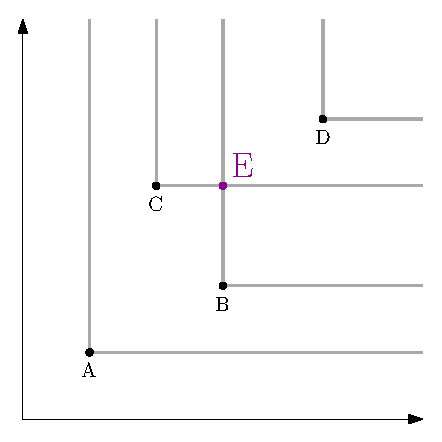
\includegraphics[scale=1]{./img/KS1.eps}
	\caption{Sample points and level sets of an examplary \ecdf.}\label{simpleEcdf}
\end{figure}


Observe, that the level sets of any \ecdf\, are uniquely determined by the sample points ( as $A, B, C$ and $D$ in Figure \ref{simpleEcdf} ) and points generated from them by taking the vectorised maximum

$$ 
	\begin{bmatrix} a_1 \cr a_2 \end{bmatrix} \vee 
	\begin{bmatrix} b_1 \cr b_2 \end{bmatrix} = 
	\begin{bmatrix} a_1 \vee b_1 \cr a_2 \vee b_2 \end{bmatrix},
$$ 
( such as $E$ in Figure \ref{simpleEcdf} ).  

One of the easiest way of establishing the values on the level sets of \Fecdf  is by considering a square, $(\nn+2)\times(\nn+2)$ matrix $B$, as in Figure \ref{spaceDivision}. The entries of $B$ correspond to values of \Fecdf\, on certain rectangles. Take the set of all $x$-coordinates of sample-points, $\Phi_x$, and the set of all $y$-coordinates of sample-points, $\Phi_y$. Add to them the coordinates of two dummy points: $(x_0, y_0)$ and $(x_{\nn+1}, y_{\nn+1})$ We enumerate points of these sets in the ascending order, $\Phi_x = \{ x_0 < x_1 < \dots <x_\nn < x_{\nn+1} \}$ and $\Phi_y = \{ y_0 < y_1 < \dots <y_\nn < y_{\nn+1} \}$. Then, the \Fecdf\, function is constant on rectangles 

$$R_{ij} = [x_i, x_{i+1})\times[y_j, y_{j+1}),$$ 
where $i,j \in \{0, 1, \dots, \nn+1 \}$. 

To actually derive the \KS\, we must assume that we can evaluate not only the true \cdf\, $F$, but also its two marginals\footnote{Limits of all the possible subsets of coordinates in infinity.}. Similarly to its univariate counterpart, the \KS\, can be calculated on only a finite number of points. Consider any rectangle. \Fecdf\, is constant on it. So the \KS depends solely on the evaluations of $F$ on that set. But $F$ is a distribuant - a function monotone in all its arguments, and so the maximum distance from \Fecdf\, can be attained only on the vertices of the rectangle. On the border rectangles ( $R_{i,\nn+1}$ and $R_{\nn+1,j}$ ) the evaluation simplifies to vertices adjacent to $R_{ij}$ rectangles and it is there, where we have to evaluate the marginals instead of $F$. \Fecdf\, is equal to zero on rectangles on the southern and western extremities. Thus we put $B_{i0} = B_{0j} = 0$. 

\begin{figure}
	\centering 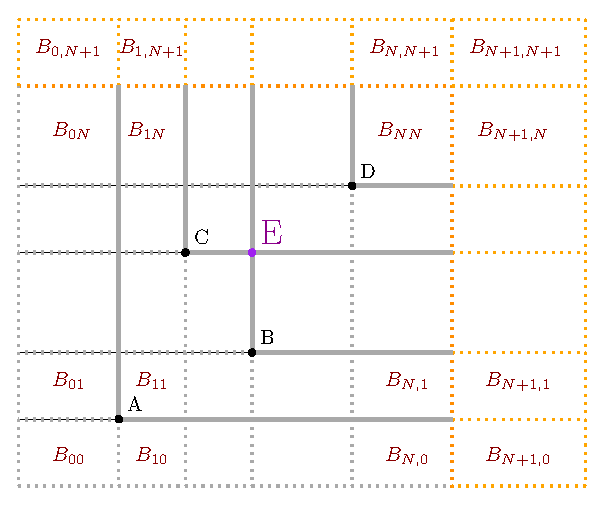
\includegraphics[scale=1]{./img/KS2.eps}
	\caption{Sample points and level sets of an examplary \ecdf.}\label{spaceDivision}
\end{figure}


The rest of the algorithm is based on the dynamic programming approach introduced by \citet*{NiVingron} for comparing lists of changes in gene expression under different scoring regimes. The overall algorithm proceeds as follows:

\begin{algorithm}
	\item Let $KS := 0$, $\jj = \nn+1$. 
	\item Read $\alpha$
	\item Prepare $\Phi_x$ and $\Phi_y$.
	\item While $i \leq \nn+1$, and while $j \in \{ 1, \dots, \ii \}$ 
	\begin{algorithm}
		\item $B_{ij} := 
			\begin{cases} 
				B_{i-1,j-1} + \text{adequate charge}, \text{ if $R_{ij}$'s upper-left vertex is a sample-point} \cr
				B_{i,j-1} + B_{i-1,j} -  B_{i-1,j-1}, \text{ Otherwise} 
			\end{cases}$	

		\item If $i,j < \nn+1$ and both $B_{ij} > B_{i,j-1} \vee B_{i-1,j}$, then evaluate $F_{ij} = F(x_i, y_j)$.

		\item If either $i$ or $j$ equals $\nn+1$ evaluate the marginal distribtion.

		\item\label{changes} Evaluate $|F_{ij} - B_{ab}|$ at $a \in \{i-1,i\}$ and $b \in \{j-1,j\}$ or only on $i-1$ and $j-1$ if on border. If it is bigger than $KS$ then update $KS$. If the update occured and the new $KS$ is such, that $F_{ij}\wedge B_{ij} > 1 - KS - \alpha$ then update $\jj$ to $j-1$.

		\item Increase $j$ by one. After the end of loop increase $i$ by one.

	\end{algorithm}
	\item Return $KS$.
\end{algorithm}

Important changes with respect to \cite{NiVingron} can be seen in point \ref{changes} and the introduction of two extra variables $\jj$ and $\alpha$. The introduction of $\jj$ stems from the easy observation, that if both distribuant $F$ and \Fecdf\, are already in the interval $(1-KS,1]$, then any further evaluations of $KS$ to the East and North could not result in a bigger difference then the one already observed. Parameter $\alpha$ gives a further reduction in the number of calculations, enlarging that band to $(1-KS-\alpha,1]$, so that the true \KS will not be larger than by $\alpha$ from the value already established. Other changes are not so important and result from discretisation of what could have seemed a continous problem. 

Our impelementation of the \KS calculator might not the optimal one. As pointed out by \citet*{Jon} the problem of calculating values of an \ecdf\, only in the sample points could be solved in $\mathcal{O}(\nn \log( \nn ))$ iterations. The existence of an algorithm requiring only $\mathcal{O}(\hat{\nn} \log( \hat{\nn}  ))$ operations, where $\hat{\nn} = \# \{ z : \exists x,y \in \text{Sample} x,y \not=z \text{ and } z = x \vee y \}$, interesting in its own sake, is left for future research.


	\chapter{ Simulations and Results }
	\chapter*{Summary and Future Research Directions}
\addcontentsline{toc}{chapter}{Summary}

As seen in the Chapter \ref{motivation} the standard Metropolis-Hastings algorithm has intrinsic limitations when it comes to solving the \ref{Problem} of drawing sample points from multimodal distributions. The \PT\, serves as a potential solution to that \ref{Problem}, being at the same time quite a flexible approach. 

In this work we have envisaged several Swapping Strategies. These Strategies are nothing else but laws according to which the \PT\, travels through the \sspace. \ref{strat1} served together with \ref{strat5} and \ref{strat6} as reference points for the remaining three strategies. \ref{strat1} is based on the idea of \textsc{PTEEM} devised by \citet{BaragattiParallelTemperingWithEquiEnergyMoves} of swaps occuring between chains that end up having the most similar temperature levels. \ref{strat5} and \ref{strat6} on the other hand are state-independent strategies, as exposed in \citet{BM2}. Two different measures have showed a slight improvement in approximating the target distribution as measured by the two-dimensional \textsc{KS} statistics and the count of undiscovered modes when using \ref{strat3}. On the other hand the criterion based on measuring approximated Average Absolute Error\footnote{Approximated by the arbitrary but reasonable choice of the sample points classifier.} has given better results when using \ref{strat1}. However all the measures yield fairly similar results in that the state-dependent strategies are better than state-independent strategies and so their use seems more than plausible when solving real life problems. 

All the necessary calculations were done using a state-of-the-are programme written in \textbf{R} statistical computation language. The implementation envisages a meticulously applied object oriented programming paradigm dictated by the modularity of the problem, as exposed in Chapter \ref{Implementation}. The modularity of the solution to the \ref{Problem} stems from instrinsic features of the Markov Chain Monte Carlo that can be better understood by the study of its more abstract mathematical formulation that underlines the possibility of using virtually any \sspace. From the statement of this fact the observation, that both the \MH\, and the \PT\, can be understood as algorithms that need as input only evaluations of different probabilities. The probability measure\footnote{With minor exception for the Quasi-Metric applied in \ref{strat4}.} is therefore the only link between the implementation of the \sspace\, and the implementation of the \algo. 

In search for some good measure of comparing different strategies, the \textsc{KS} statistics was given appropriate attention. Because of the lack of a R-implemented software, a new implementation was derived, based on approach derived by \citet{NiVingron}, with minor improvements that prevent from unnecessary calculations.

All of the implemented software is to be shiped soon as an independent \textbf{R} package.           

As for the future plans an implementation of an adaptive version of the \PT\, is planned. The need for such algorithm stems from a potential drawback in the \PT, which is the lack of a unified approach to setting up the temperature levels. In fact the internalisation of such procedures into the algorithmic model could enhance mightly the efficiency parameters of the algorithm, e.g. by reduction in the number of unnecessary chains. 

We also think that implementation of the \textsc{KS} calculator can be significanlty improved by meticulous application of the multi-dimensional {\it divide et impera} approach, originally developed by \citet{Jon}.  

Moreover, for technical reasons the derived template should be re-implemented using a faster and more orderly computer language, such as \textbf{C++}.

	\bibliographystyle{./bibliography/eccaNoNotes}
	\bibliography{./bibliography/myBooks}

\end{document}